% Standalone formulation of the implemented October 14 local-dynamics method.
% Compile twice with pdflatex. No external files are required.
\documentclass[11pt,a4paper]{article}
\usepackage[T1]{fontenc}
\usepackage[utf8]{inputenc}
\usepackage{lmodern}
\usepackage[margin=24mm,headheight=14pt]{geometry}
\usepackage{amsmath,amssymb,mathtools}
\usepackage{booktabs,tabularx,array}
\usepackage{microtype}
\usepackage{fancyhdr}
\usepackage[hidelinks]{hyperref}
\hypersetup{pdftitle={Learning Local Structure and Motion from Simulation},pdfauthor={},pdfsubject={Problem formulation and method}}
\numberwithin{equation}{section}
\newcommand{\R}{\mathbb R}
\newcommand{\Sim}{\operatorname{Sim}}
\newcommand{\Local}{\operatorname{Local}}
\newcommand{\MSE}{\operatorname{MSE}}
\newcommand{\sg}{\operatorname{stopgrad}}
\newcommand{\mean}{\operatorname{mean}}
\newcommand{\asinh}{\operatorname{asinh}}
\newcommand{\softmax}{\operatorname{softmax}}
\newcommand{\sm}{\mathrm{sm}}
\newcommand{\vel}{\mathrm{vel}}
\newcommand{\dd}{\,\mathrm d}
\setlength{\parindent}{0pt}
\setlength{\parskip}{0.3em}
\setlength{\emergencystretch}{2.5em}
\pagestyle{fancy}\fancyhf{}
\fancyhead[L]{\small Learning local structure and motion}
\fancyfoot[C]{\small\thepage}
\renewcommand{\headrulewidth}{0.3pt}
\widowpenalty=10000\clubpenalty=10000
\title{\vspace{-1.5em}\Large\bfseries Learning Local Structure and Motion from Simulation}
\author{}\date{}

% All three diagrams are editable TikZ; no external image files are used.
\usepackage{tikz}
\usetikzlibrary{arrows.meta,calc,positioning}
\usepackage[font=small,labelfont=bf]{caption}
% Shared figure typography and restrained print palette.
\definecolor{pcmInk}{HTML}{242424}
\definecolor{pcmBlue}{HTML}{315E8A}
\definecolor{pcmGreen}{HTML}{287668}
\definecolor{pcmAmber}{HTML}{9B632D}
\definecolor{pcmGray}{HTML}{505050}
\definecolor{pcmRule}{HTML}{A0A0A0}
\tikzset{
  pcm/base/.style={rectangle,line width=.4pt,
    align=center,inner xsep=4pt,inner ysep=5pt,outer sep=1pt,
    font=\rmfamily\fontsize{9.4}{11.8}\selectfont,
    text=pcmInk,execute at begin node={\hyphenpenalty=10000\exhyphenpenalty=10000}},
  pcm/model/.style={pcm/base,draw=pcmBlue!75,fill=pcmBlue!3},
  pcm/physical/.style={pcm/base,draw=pcmGreen!75,fill=pcmGreen!3},
  pcm/loss/.style={pcm/base,draw=none,fill=none},
  pcm/context/.style={pcm/base,draw=none,fill=none},
  pcm/text/.style={align=center,inner sep=0pt,text=pcmInk,
    font=\rmfamily\fontsize{9.4}{11.8}\selectfont},
  pcm/small/.style={pcm/text,font=\rmfamily\fontsize{8.6}{10.8}\selectfont},
  pcm/head/.style={anchor=west,inner sep=0pt,text=pcmInk,
    font=\rmfamily\bfseries\fontsize{10.4}{12.4}\selectfont},
  pcm/arrow/.style={-{Latex[length=1.5mm,width=1.1mm]},line width=.45pt,draw=pcmGray},
  pcm/bluearrow/.style={pcm/arrow,draw=pcmBlue},
  pcm/greenarrow/.style={pcm/arrow,draw=pcmGreen},
  pcm/amberarrow/.style={pcm/arrow,draw=pcmAmber},
  pcm/wire/.style={line width=.45pt,draw=pcmBlue}
}
\newsavebox{\pcmFigureBox}
\newcommand{\PlacePCMDiagram}[1]{%
  \sbox{\pcmFigureBox}{#1}%
  \typeout{PCM-DIAGRAM width=\the\wd\pcmFigureBox; height=\the\ht\pcmFigureBox; depth=\the\dp\pcmFigureBox}%
  \ifdim\wd\pcmFigureBox>\linewidth
    \PackageError{pcmfigures}{Diagram exceeds text width}{Reduce diagram geometry, not the document margins.}%
  \fi
  \usebox{\pcmFigureBox}%
}
\makeatletter
\setlength{\@fptop}{0pt}
\makeatother
\renewcommand{\floatpagefraction}{.65}
\setlength{\textfloatsep}{15pt plus 2pt minus 2pt}
\setlength{\intextsep}{15pt plus 2pt minus 2pt}
% Geometry logging for render-time layout checks.
\newcommand{\PCMLogNode}[1]{\begingroup
  \pgfextractx{\dimen0}{\pgfpointanchor{#1}{south west}}%
  \pgfextracty{\dimen2}{\pgfpointanchor{#1}{south west}}%
  \pgfextractx{\dimen4}{\pgfpointanchor{#1}{north east}}%
  \pgfextracty{\dimen6}{\pgfpointanchor{#1}{north east}}%
  \typeout{PCM-NODE|#1|\the\dimen0|\the\dimen2|\the\dimen4|\the\dimen6}%
\endgroup}

% Figure 1: overview. Vertical layout avoids crossing loss connections.
\newcommand{\PCMOverviewDiagram}{%
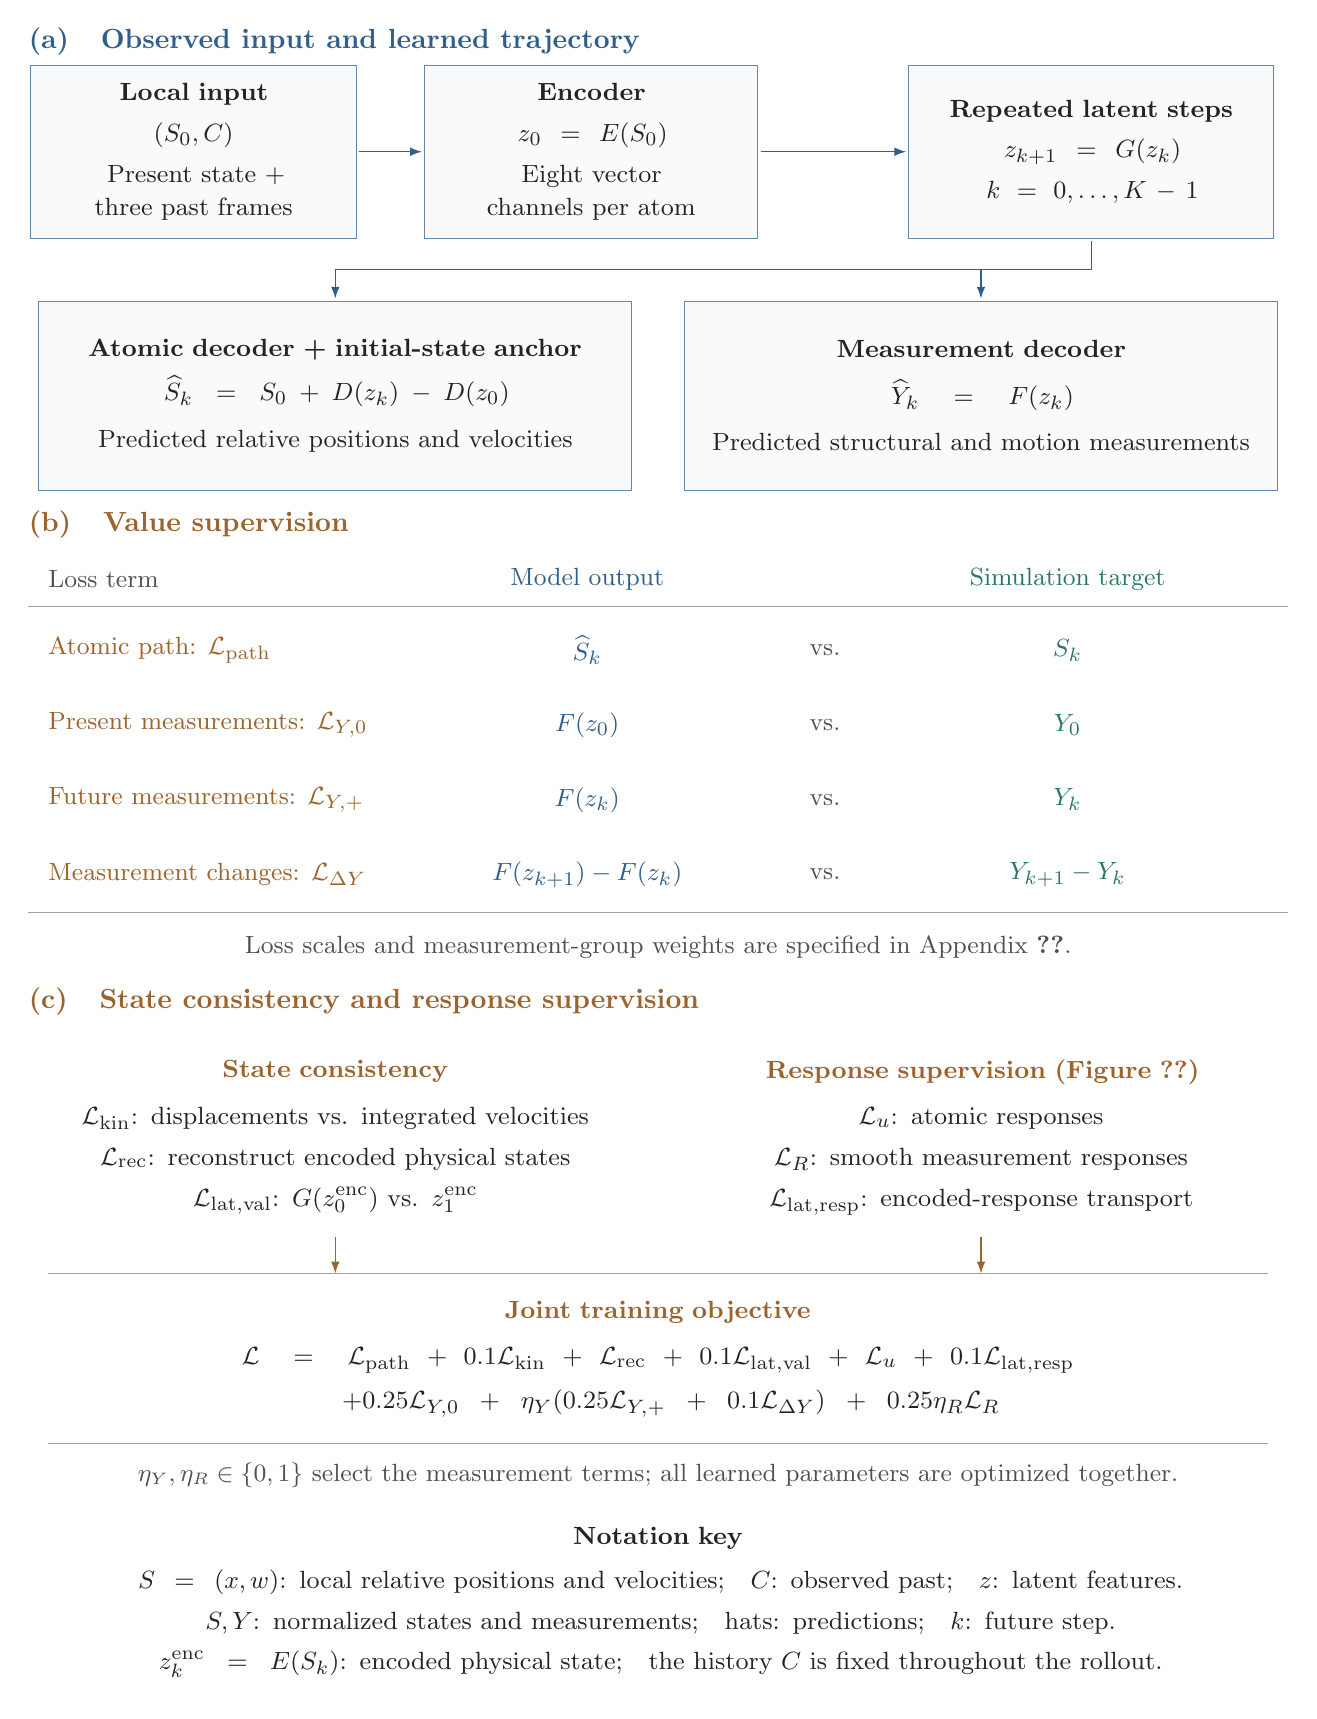
\begin{tikzpicture}[x=1cm,y=1cm]
  \node[pcm/head,text=pcmBlue] at (0,21.05)
    {(a)\quad Observed input and learned trajectory};
  \node[pcm/model,text width=3.85cm,minimum height=2.20cm] (ov-input) at (2.10,19.65)
    {\textbf{Local input}\\[3pt]
     $(S_0,C)$\\[3pt]
     Present state + three past frames};
  \node[pcm/model,text width=3.95cm,minimum height=2.20cm] (ov-encoder) at (7.15,19.65)
    {\textbf{Encoder}\\[3pt]
     $z_0=E(S_0)$\\[3pt]
     Eight vector channels per atom};
  \node[pcm/model,text width=4.35cm,minimum height=2.20cm] (ov-rollout) at (13.50,19.65)
    {\textbf{Repeated latent steps}\\[3pt]
     $z_{k+1}=G(z_k)$\\[3pt]
     $k=0,\ldots,K-1$};
  \draw[pcm/bluearrow] (ov-input.east) -- (ov-encoder.west);
  \draw[pcm/bluearrow] (ov-encoder.east) -- (ov-rollout.west);

  \node[pcm/model,text width=7.25cm,minimum height=2.40cm] (ov-atomic) at (3.90,16.55)
    {\textbf{Atomic decoder + initial-state anchor}\\[4pt]
     $\widehat S_k=S_0+D(z_k)-D(z_0)$\\[5pt]
     Predicted relative positions and velocities};
  \node[pcm/model,text width=7.25cm,minimum height=2.40cm] (ov-measurement) at (12.10,16.55)
    {\textbf{Measurement decoder}\\[5pt]
     $\widehat Y_k=F(z_k)$\\[5pt]
     Predicted structural and motion measurements};
  \draw[pcm/wire] (ov-rollout.south) -- (13.50,18.15) -- (3.90,18.15);
  \draw[pcm/bluearrow] (3.90,18.15) -- (ov-atomic.north);
  \draw[pcm/bluearrow] (12.10,18.15) -- (ov-measurement.north);

  \node[pcm/head,text=pcmAmber] at (0,14.92)
    {(b)\quad Value supervision};
  \node[pcm/small,anchor=west,text=pcmGray] at (.25,14.22) {Loss term};
  \node[pcm/small,text=pcmBlue] at (7.10,14.22) {Model output};
  \node[pcm/small,text=pcmGreen] at (13.20,14.22) {Simulation target};
  \draw[pcmRule] (0,13.87) -- (16,13.87);
  \node[pcm/text,anchor=west,text=pcmAmber] at (.25,13.32)
    {Atomic path: $\mathcal L_{\rm path}$};
  \node[pcm/text,text=pcmBlue] at (7.10,13.32) {$\widehat S_{k}$};
  \node[pcm/small,text=pcmGray] at (10.12,13.32) {vs.};
  \node[pcm/text,text=pcmGreen] at (13.20,13.32) {$S_k$};
  \node[pcm/text,anchor=west,text=pcmAmber] at (.25,12.37)
    {Present measurements: $\mathcal L_{Y,0}$};
  \node[pcm/text,text=pcmBlue] at (7.10,12.37) {$F(z_0)$};
  \node[pcm/small,text=pcmGray] at (10.12,12.37) {vs.};
  \node[pcm/text,text=pcmGreen] at (13.20,12.37) {$Y_0$};
  \node[pcm/text,anchor=west,text=pcmAmber] at (.25,11.42)
    {Future measurements: $\mathcal L_{Y,+}$};
  \node[pcm/text,text=pcmBlue] at (7.10,11.42) {$F(z_k)$};
  \node[pcm/small,text=pcmGray] at (10.12,11.42) {vs.};
  \node[pcm/text,text=pcmGreen] at (13.20,11.42) {$Y_k$};
  \node[pcm/text,anchor=west,text=pcmAmber] at (.25,10.47)
    {Measurement changes: $\mathcal L_{\Delta Y}$};
  \node[pcm/text,text=pcmBlue] at (7.10,10.47) {$F(z_{k+1})-F(z_k)$};
  \node[pcm/small,text=pcmGray] at (10.12,10.47) {vs.};
  \node[pcm/text,text=pcmGreen] at (13.20,10.47) {$Y_{k+1}-Y_k$};
  \draw[pcmRule] (0,9.99) -- (16,9.99);
  \node[pcm/small,text=pcmGray] at (8,9.55)
    {Loss scales and measurement-group weights are specified in Appendix~\ref{app:normalization}.};

  \node[pcm/head,text=pcmAmber] at (0,8.86)
    {(c)\quad State consistency and response supervision};
  \node[pcm/loss,text width=7.25cm,minimum height=2.45cm] (ov-state-loss) at (3.90,7.13)
    {\textcolor{pcmAmber}{\textbf{State consistency}}\\[5pt]
     $\mathcal L_{\rm kin}$: displacements vs. integrated velocities\\[3pt]
     $\mathcal L_{\rm rec}$: reconstruct encoded physical states\\[3pt]
     $\mathcal L_{\rm lat,val}$: $G(z_0^{\rm enc})$ vs. $z_1^{\rm enc}$};
  \node[pcm/loss,text width=7.25cm,minimum height=2.45cm] (ov-response-loss) at (12.10,7.13)
    {\textcolor{pcmAmber}{\textbf{Response supervision (Figure~\ref{fig:response-supervision})}}\\[5pt]
     $\mathcal L_u$: atomic responses\\[3pt]
     $\mathcal L_R$: smooth measurement responses\\[3pt]
     $\mathcal L_{\rm lat,resp}$: encoded-response transport};

  \draw[pcmAmber!65,line width=.4pt] (.25,5.40) -- (15.75,5.40);
  \draw[pcmAmber!65,line width=.4pt] (.25,3.24) -- (15.75,3.24);
  \node[pcm/loss,text width=15.45cm,minimum height=2.10cm] (ov-joint) at (8,4.32)
    {\textcolor{pcmAmber}{\textbf{Joint training objective}}\\[5pt]
     $\mathcal L=\mathcal L_{\rm path}+0.1\mathcal L_{\rm kin}+\mathcal L_{\rm rec}
      +0.1\mathcal L_{\rm lat,val}+\mathcal L_u+0.1\mathcal L_{\rm lat,resp}$\\[4pt]
     $\quad+0.25\mathcal L_{Y,0}
      +\eta_Y(0.25\mathcal L_{Y,+}+0.1\mathcal L_{\Delta Y})
      +0.25\eta_R\mathcal L_R$};
  \draw[pcm/amberarrow] (ov-state-loss.south) -- (ov-joint.north -| ov-state-loss.south);
  \draw[pcm/amberarrow] (ov-response-loss.south) -- (ov-joint.north -| ov-response-loss.south);
  \node[pcm/small,text=pcmGray] at (8,2.84)
    {$\eta_Y,\eta_R\in\{0,1\}$ select the measurement terms; all learned parameters are optimized together.};

  \node[pcm/context,text width=15.45cm,minimum height=2.20cm] at (8,1.23)
    {\textbf{Notation key}\\[4pt]
     $S=(x,w)$: local relative positions and velocities;\quad $C$: observed past;\quad $z$: latent features.\\[3pt]
     $S,Y$: normalized states and measurements;\quad hats: predictions;\quad $k$: future step.\\[3pt]
     $z_k^{\rm enc}=E(S_k)$: encoded physical state;\quad the history $C$ is fixed throughout the rollout.};
\PCMLogNode{ov-input}
\PCMLogNode{ov-encoder}
\PCMLogNode{ov-rollout}
\PCMLogNode{ov-atomic}
\PCMLogNode{ov-measurement}
\PCMLogNode{ov-state-loss}
\PCMLogNode{ov-response-loss}
\PCMLogNode{ov-joint}
\end{tikzpicture}%
}

% Figure 2: full system -> local positions/velocities -> fixed measurements.
\newcommand{\PCMLocalDiagram}{%
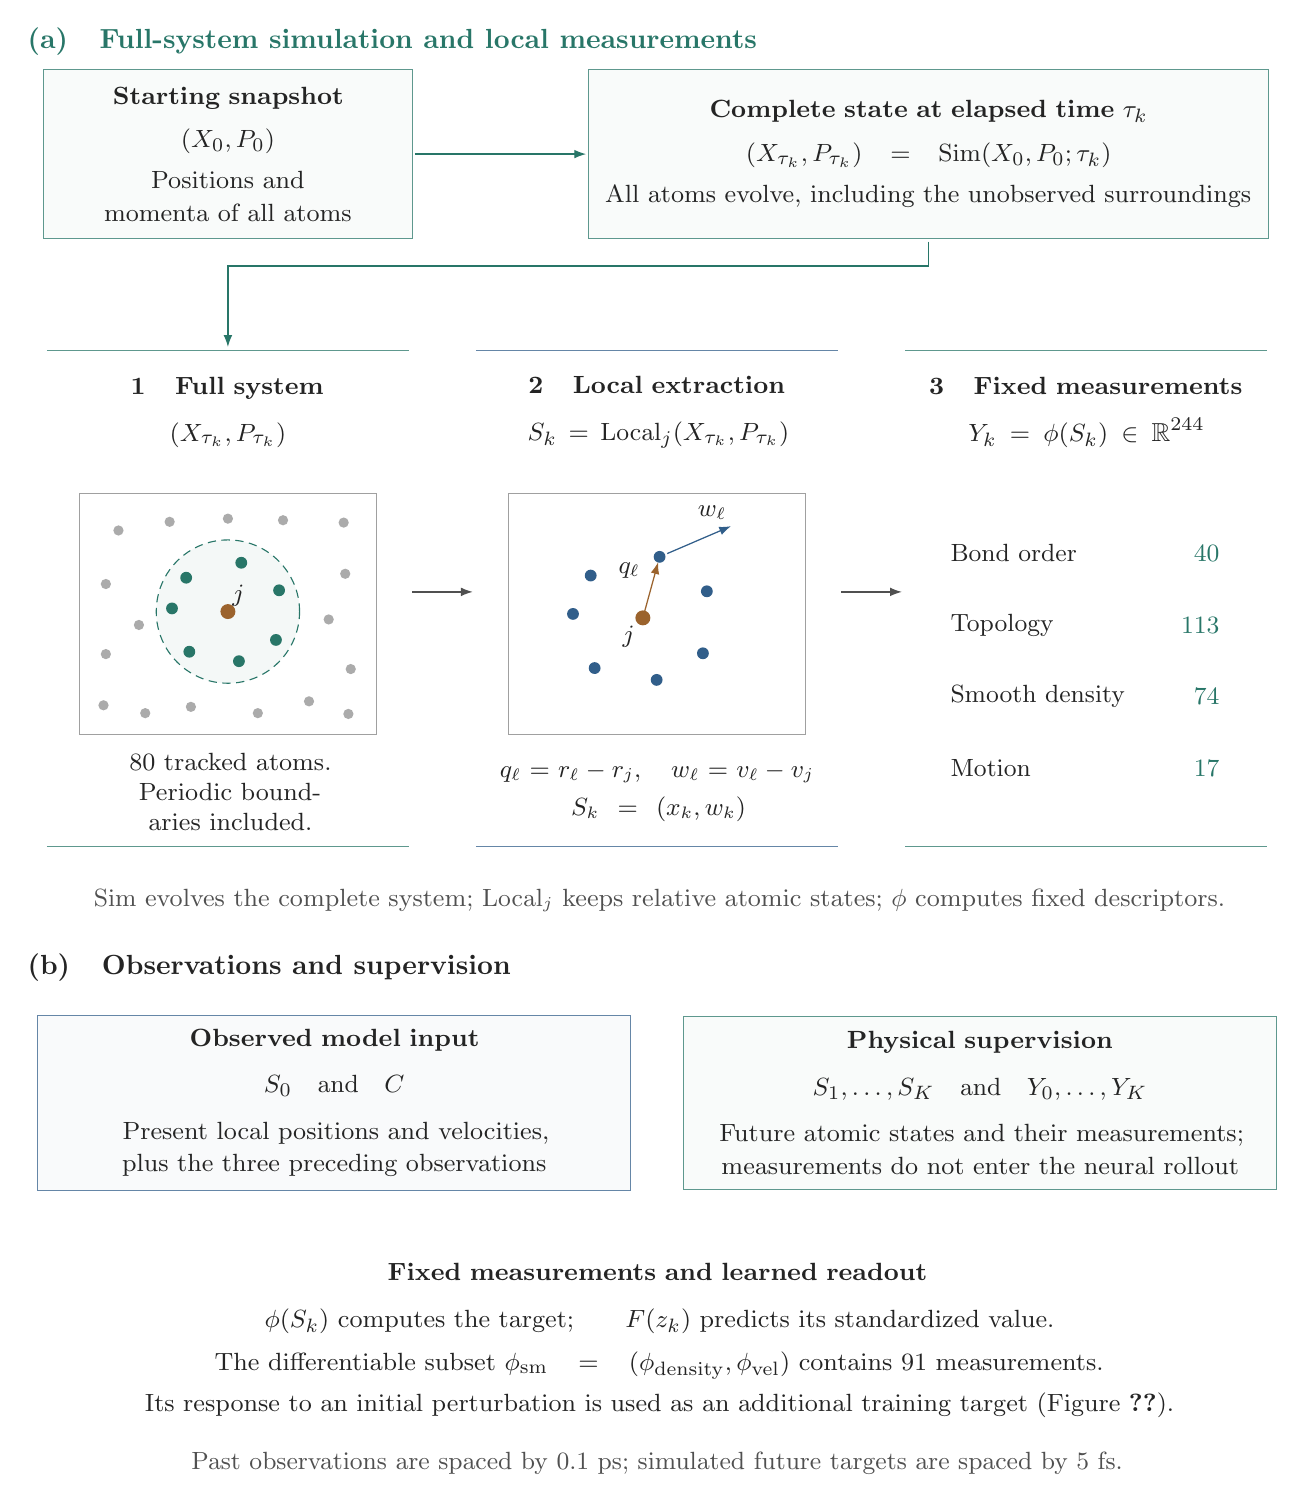
\begin{tikzpicture}[x=1cm,y=1cm]
  \node[pcm/head,text=pcmGreen] at (0,19.15)
    {(a)\quad Full-system simulation and local measurements};
  \node[pcm/physical,text width=4.40cm,minimum height=2.15cm] (lc-initial) at (2.55,17.72)
    {\textbf{Starting snapshot}\\[4pt]
     $(X_0,P_0)$\\[3pt]
     Positions and momenta of all atoms};
  \node[pcm/physical,text width=8.35cm,minimum height=2.15cm] (lc-simulation) at (11.45,17.72)
    {\textbf{Complete state at elapsed time $\tau_k$}\\[4pt]
     $(X_{\tau_k},P_{\tau_k})=\Sim(X_0,P_0;\tau_k)$\\[3pt]
     All atoms evolve, including the unobserved surroundings};
  \draw[pcm/greenarrow] (lc-initial.east) -- (lc-simulation.west);
  \draw[pcm/greenarrow] (lc-simulation.south) -- (11.45,16.30)
     -- (2.55,16.30) -- (2.55,15.27);

  % Three open panels, separated by short horizontal rules.
  \foreach \left/\right/\tint in {.25/4.85/pcmGreen,5.70/10.30/pcmBlue,11.15/15.75/pcmGreen}{
    \draw[\tint!75,line width=.4pt] (\left,15.23) -- (\right,15.23);
    \draw[\tint!75,line width=.4pt] (\left,8.93) -- (\right,8.93);
  }
  \node[pcm/text,text width=4.10cm] at (2.55,14.44)
    {\textbf{1\quad Full system}\\[5pt]$(X_{\tau_k},P_{\tau_k})$};
  \node[pcm/text,text width=4.10cm] at (8.00,14.44)
    {\textbf{2\quad Local extraction}\\[5pt]$S_k=\Local_j(X_{\tau_k},P_{\tau_k})$};
  \node[pcm/text,text width=4.10cm] at (13.45,14.44)
    {\textbf{3\quad Fixed measurements}\\[5pt]$Y_k=\phi(S_k)\in\R^{244}$};
  \draw[pcm/arrow] (4.89,12.16) -- (5.66,12.16);
  \draw[pcm/arrow] (10.34,12.16) -- (11.11,12.16);

  % Full-system sketch: grey exterior, green selected atoms, highlighted center.
  \draw[pcmRule,fill=white,line width=.4pt] (.66,10.35) rectangle (4.44,13.41);
  \fill[pcmGreen!5] (2.55,11.91) circle [radius=.91];
  \draw[pcmGreen,densely dashed,line width=.4pt] (2.55,11.91) circle [radius=.91];
  \foreach \xx/\yy in {.97/10.72,1.50/10.62,2.08/10.70,2.93/10.62,3.58/10.77,4.08/10.61,
    1.00/11.37,1.42/11.74,1.00/12.26,1.16/12.94,1.81/13.05,2.55/13.09,
    3.25/13.07,4.02/13.04,4.04/12.39,3.83/11.81,4.11/11.18}{
    \fill[pcmGray!48] (\xx,\yy) circle [radius=.065];
  }
  \foreach \xx/\yy in {2.02/12.34,2.72/12.53,3.20/12.18,3.16/11.55,
    2.69/11.28,2.06/11.40,1.84/11.95}{
    \fill[pcmGreen] (\xx,\yy) circle [radius=.075];
  }
  \fill[pcmAmber] (2.55,11.91) circle [radius=.095];
  \node[pcm/small,anchor=south west,text=pcmInk] at (2.60,11.97) {$j$};
  \node[pcm/small,text width=4.02cm] at (2.55,9.62)
    {80 tracked atoms.\\Periodic boundaries included.};

  % Local sketch, with a relative displacement and a relative velocity.
  \draw[pcmRule,fill=white,line width=.4pt] (6.11,10.35) rectangle (9.89,13.41);
  \foreach \xx/\yy in {7.1575/12.3675,8.0325/12.605,8.6325/12.1675,8.5825/11.38,7.995/11.0425,7.2075/11.1925,6.9325/11.88}{
    \fill[pcmBlue] (\xx,\yy) circle [radius=.075];
  }
  \fill[pcmAmber] (7.82,11.83) circle [radius=.095];
  \node[pcm/small,anchor=north east,text=pcmInk] at (7.72,11.73) {$j$};
  \draw[pcm/arrow,draw=pcmAmber,shorten >=2pt] (7.82,11.83) -- (8.0325,12.605);
  \node[pcm/small,text=pcmInk,anchor=east] at (7.79,12.43) {$q_\ell$};
  \draw[pcm/bluearrow,shorten <=3pt] (8.0325,12.605) -- (8.94,12.995);
  \node[pcm/small,text=pcmInk,anchor=south] at (8.70,13.07) {$w_\ell$};
  \node[pcm/small,text width=4.20cm] at (8.00,9.62)
    {$q_\ell=r_\ell-r_j,\quad w_\ell=v_\ell-v_j$\\[3pt]
     $S_k=(x_k,w_k)$};

  % Four fixed measurement groups.
  \foreach \yy/\labeltext/\number in {12.65/Bond order/40,11.74/Topology/113,10.83/Smooth density/74,9.92/Motion/17}{
    \node[pcm/text,anchor=west] at (11.72,\yy) {\labeltext};
    \node[pcm/text,anchor=east,text=pcmGreen] at (15.15,\yy) {\number};
  }

  \node[pcm/small,text width=15.50cm,text=pcmGray] at (8,8.24)
    {$\Sim$ evolves the complete system; $\Local_j$ keeps relative atomic states; $\phi$ computes fixed descriptors.};
  \node[pcm/head] at (0,7.39)
    {(b)\quad Observations and supervision};
  \node[pcm/model,text width=7.25cm,minimum height=2.20cm] (lc-model-input) at (3.90,5.67)
    {\textbf{Observed model input}\\[5pt]
     $S_0\quad\text{and}\quad C$\\[5pt]
     Present local positions and velocities,\\plus the three preceding observations};
  \node[pcm/physical,text width=7.25cm,minimum height=2.20cm] (lc-supervision) at (12.10,5.67)
    {\textbf{Physical supervision}\\[5pt]
     $S_1,\ldots,S_K\quad\text{and}\quad Y_0,\ldots,Y_K$\\[5pt]
     Future atomic states and their measurements;\\measurements do not enter the neural rollout};

  \node[pcm/context,text width=15.45cm,minimum height=1.80cm] (lc-key) at (8,2.65)
    {\textbf{Fixed measurements and learned readout}\\[5pt]
     $\phi(S_k)$ computes the target;\qquad $F(z_k)$ predicts its standardized value.\\[4pt]
     The differentiable subset $\phi_{\sm}=(\phi_{\rm density},\phi_{\vel})$ contains 91 measurements.\\[3pt]
     Its response to an initial perturbation is used as an additional training target (Figure~\ref{fig:response-supervision}).};
  \node[pcm/small,text=pcmGray] at (8,1.09)
    {Past observations are spaced by 0.1 ps; simulated future targets are spaced by 5 fs.};
\PCMLogNode{lc-initial}
\PCMLogNode{lc-simulation}
\PCMLogNode{lc-model-input}
\PCMLogNode{lc-supervision}
\PCMLogNode{lc-key}
\end{tikzpicture}%
}

% Figure 3: physical response matching and latent tangent transport.
\newcommand{\PCMResponseDiagram}{%
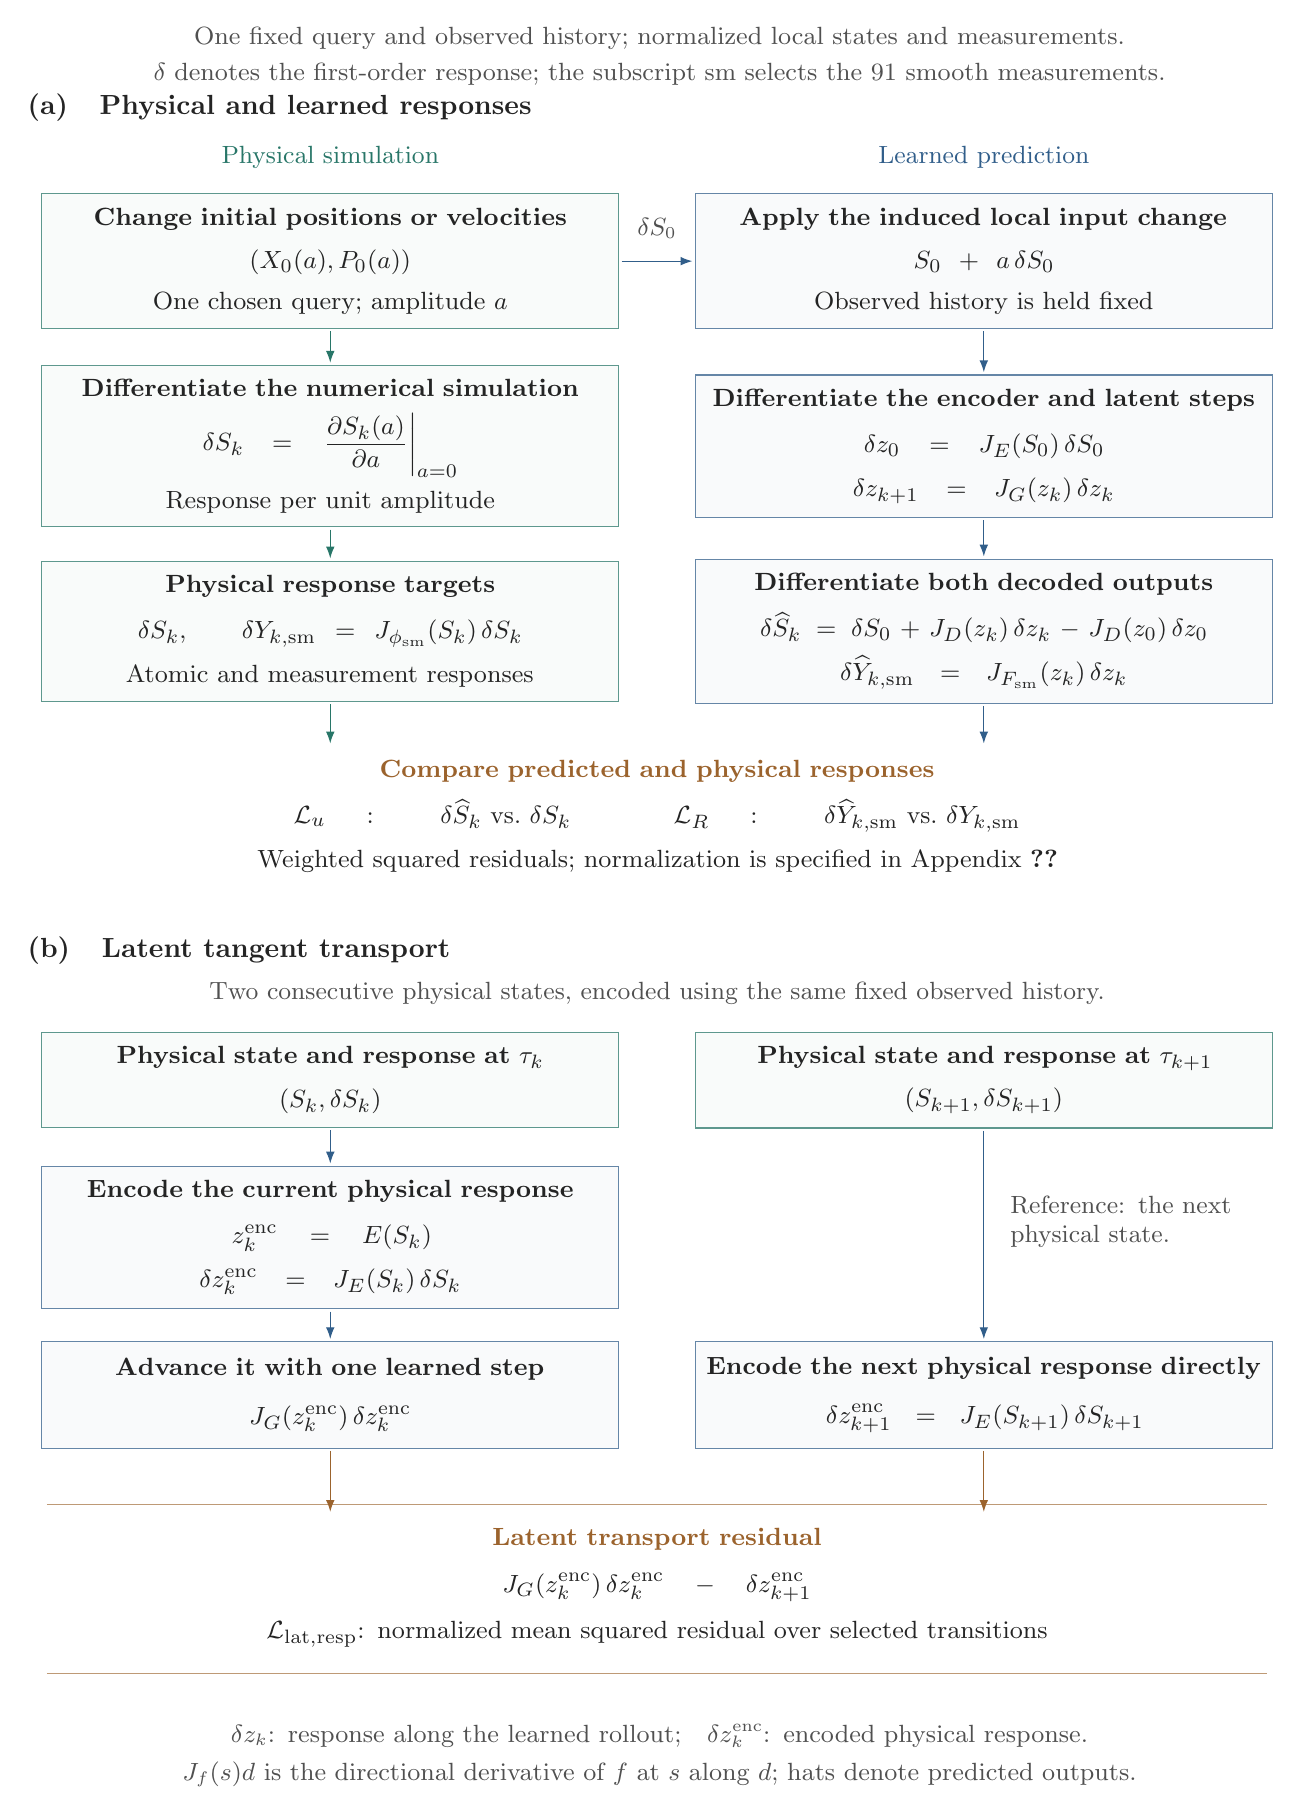
\begin{tikzpicture}[x=1cm,y=1cm]
  \node[pcm/small,text width=15.5cm,text=pcmGray] at (8,22.30)
    {One fixed query and observed history; normalized local states and measurements.\\[2pt]
     $\delta$ denotes the first-order response; the subscript $\sm$ selects the 91 smooth measurements.};
  \node[pcm/head] at (0,21.65)
    {(a)\quad Physical and learned responses};
  \node[pcm/small,text=pcmGreen] at (3.85,21.02) {Physical simulation};
  \node[pcm/small,text=pcmBlue] at (12.15,21.02) {Learned prediction};
  \node[pcm/physical,text width=7.05cm,minimum height=1.55cm] (rp-query) at (3.85,19.70)
    {\textbf{Change initial positions or velocities}\\[4pt]
     $(X_0(a),P_0(a))$\\[3pt]
     One chosen query; amplitude $a$};
  \node[pcm/model,text width=7.05cm,minimum height=1.55cm] (rp-input) at (12.15,19.70)
    {\textbf{Apply the induced local input change}\\[4pt]
     $S_0+a\,\delta S_0$\\[3pt]
     Observed history is held fixed};
  \draw[pcm/bluearrow] (rp-query.east) -- (rp-input.west);
  \node[pcm/small,text=pcmGray] at (8,20.12) {$\delta S_0$};

  \node[pcm/physical,text width=7.05cm,minimum height=1.75cm] (rp-physical-derivative) at (3.85,17.35)
    {\textbf{Differentiate the numerical simulation}\\[5pt]
     $\delta S_k=\left.\dfrac{\partial S_k(a)}{\partial a}\right|_{a=0}$\\[4pt]
     Response per unit amplitude};
  \node[pcm/model,text width=7.05cm,minimum height=1.75cm] (rp-latent) at (12.15,17.35)
    {\textbf{Differentiate the encoder and latent steps}\\[5pt]
     $\delta z_0=J_E(S_0)\,\delta S_0$\\[4pt]
     $\delta z_{k+1}=J_G(z_k)\,\delta z_k$};
  \draw[pcm/greenarrow] (rp-query.south) -- (rp-physical-derivative.north);
  \draw[pcm/bluearrow] (rp-input.south) -- (rp-latent.north);

  \node[pcm/physical,text width=7.05cm,minimum height=1.65cm] (rp-targets) at (3.85,15.00)
    {\textbf{Physical response targets}\\[5pt]
     $\delta S_k,\qquad \delta Y_{k,\sm}=J_{\phi_{\sm}}(S_k)\,\delta S_k$\\[4pt]
     Atomic and measurement responses};
  \node[pcm/model,text width=7.05cm,minimum height=1.65cm] (rp-predictions) at (12.15,15.00)
    {\textbf{Differentiate both decoded outputs}\\[5pt]
     $\delta\widehat S_k=\delta S_0+J_D(z_k)\,\delta z_k-J_D(z_0)\,\delta z_0$\\[4pt]
     $\delta\widehat Y_{k,\sm}=J_{F_{\sm}}(z_k)\,\delta z_k$};
  \draw[pcm/greenarrow] (rp-physical-derivative.south) -- (rp-targets.north);
  \draw[pcm/bluearrow] (rp-latent.south) -- (rp-predictions.north);

  \node[pcm/loss,text width=15.40cm,minimum height=1.50cm] (rp-match) at (8,12.65)
    {\textcolor{pcmAmber}{\textbf{Compare predicted and physical responses}}\\[5pt]
     $\mathcal L_u:\quad\delta\widehat S_k\ \text{vs.}\ \delta S_k
     \qquad\qquad
     \mathcal L_R:\quad\delta\widehat Y_{k,\sm}\ \text{vs.}\ \delta Y_{k,\sm}$\\[4pt]
     Weighted squared residuals; normalization is specified in Appendix~\ref{app:normalization}};
  \draw[pcm/greenarrow] (rp-targets.south) -- (rp-match.north -| rp-targets.south);
  \draw[pcm/bluearrow] (rp-predictions.south) -- (rp-match.north -| rp-predictions.south);

  \node[pcm/head] at (0,10.95)
    {(b)\quad Latent tangent transport};
  \node[pcm/small,text=pcmGray] at (8,10.40)
    {Two consecutive physical states, encoded using the same fixed observed history.};
  \node[pcm/physical,text width=7.05cm,minimum height=1.05cm] (rp-current) at (3.85,9.30)
    {\textbf{Physical state and response at $\tau_k$}\\[4pt]
     $(S_k,\delta S_k)$};
  \node[pcm/physical,text width=7.05cm,minimum height=1.05cm] (rp-next) at (12.15,9.30)
    {\textbf{Physical state and response at $\tau_{k+1}$}\\[4pt]
     $(S_{k+1},\delta S_{k+1})$};

  \node[pcm/model,text width=7.05cm,minimum height=1.48cm] (rp-encoded) at (3.85,7.30)
    {\textbf{Encode the current physical response}\\[5pt]
     $z_k^{\rm enc}=E(S_k)$\\[4pt]
     $\delta z_k^{\rm enc}=J_E(S_k)\,\delta S_k$};
  \draw[pcm/bluearrow] (rp-current.south) -- (rp-encoded.north);

  \node[pcm/model,text width=7.05cm,minimum height=1.35cm] (rp-transport) at (3.85,5.30)
    {\textbf{Advance it with one learned step}\\[6pt]
     $J_G(z_k^{\rm enc})\,\delta z_k^{\rm enc}$};
  \node[pcm/model,text width=7.05cm,minimum height=1.35cm] (rp-reference) at (12.15,5.30)
    {\textbf{Encode the next physical response directly}\\[6pt]
     $\delta z_{k+1}^{\rm enc}=J_E(S_{k+1})\,\delta S_{k+1}$};
  \draw[pcm/bluearrow] (rp-encoded.south) -- (rp-transport.north);
  \draw[pcm/bluearrow] (rp-next.south) -- (rp-reference.north);
  \node[pcm/small,anchor=west,text width=2.95cm,align=left,text=pcmGray] at (12.48,7.50)
    {Reference: the next\\physical state.};

  \draw[pcmAmber!65,line width=.4pt] (.25,3.91) -- (15.75,3.91);
  \draw[pcmAmber!65,line width=.4pt] (.25,1.76) -- (15.75,1.76);
  \node[pcm/loss,text width=15.40cm,minimum height=1.80cm] (rp-transport-loss) at (8,2.85)
    {\textcolor{pcmAmber}{\textbf{Latent transport residual}}\\[5pt]
     $J_G(z_k^{\rm enc})\,\delta z_k^{\rm enc}-\delta z_{k+1}^{\rm enc}$\\[5pt]
     $\mathcal L_{\rm lat,resp}$: normalized mean squared residual over selected transitions};
  \draw[pcm/amberarrow] (rp-transport.south) -- (rp-transport-loss.north -| rp-transport.south);
  \draw[pcm/amberarrow] (rp-reference.south) -- (rp-transport-loss.north -| rp-reference.south);

  \node[pcm/small,text width=15.50cm,text=pcmGray] at (8,.72)
    {$\delta z_k$: response along the learned rollout;\quad
     $\delta z_k^{\rm enc}$: encoded physical response.\\[3pt]
     $J_f(s)d$ is the directional derivative of $f$ at $s$ along $d$; hats denote predicted outputs.};
\PCMLogNode{rp-query}
\PCMLogNode{rp-input}
\PCMLogNode{rp-physical-derivative}
\PCMLogNode{rp-latent}
\PCMLogNode{rp-targets}
\PCMLogNode{rp-predictions}
\PCMLogNode{rp-match}
\PCMLogNode{rp-current}
\PCMLogNode{rp-next}
\PCMLogNode{rp-encoded}
\PCMLogNode{rp-transport}
\PCMLogNode{rp-reference}
\PCMLogNode{rp-transport-loss}
\end{tikzpicture}%
}

\begin{document}
\setlength{\abovedisplayskip}{9pt plus 2pt minus 2pt}
\setlength{\belowdisplayskip}{9pt plus 2pt minus 2pt}
\setlength{\abovedisplayshortskip}{3pt plus 2pt}
\setlength{\belowdisplayshortskip}{6pt plus 2pt minus 2pt}
\maketitle\vspace{-2.4em}\thispagestyle{plain}

We learn a representation of a central atom and its local neighborhood from
short molecular-dynamics trajectories. The model encodes observed positions,
velocities, and recent history, advances an atom-resolved latent state, and
predicts both atomic motion and physical measurements. Training also uses
the responses of these quantities to small changes of the initial positions
or velocities. These responses constrain how the learned dynamics changes
in a neighborhood of each observed trajectory.

Figure~\ref{fig:method-overview} summarizes the inputs, outputs, and loss terms.

\begin{figure}[p]
\centering
\PlacePCMDiagram{\PCMOverviewDiagram}
\caption{\textbf{Inputs, predictions, and the training objective.}
Blue marks learned operations, green physical targets, and ochre loss terms.
The arrows in panel (a) describe prediction. Panels (b)--(c) list the comparisons that form the loss,
without adding physical targets to the model's input. The atomic output includes the
initial-state anchor. Local states and measurements use the normalized coordinates of Section~2. The fixed observed history conditions the encoder, transition, and atomic decoder.}
\label{fig:method-overview}
\end{figure}

\section{Problem formulation}

\subsection{Starting snapshots and physical time}

Starting snapshots are indexed by $i$, and $t_i$ is the physical time of
snapshot $i$ within its source trajectory. The index $j$ identifies a selected
central atom, and $\ell$ identifies an atom in its neighborhood. A local
training example is specified by $(i,j)$. Dataset ordering does not determine
physical time.

The observed history contains three preceding snapshots, spaced by
$\Delta t=0.1$ ps. A simulated continuation provides future targets every
$h=0.005$ ps, or 5 fs. We index these targets by $k$ and write
\begin{equation}
\tau_k=kh,\qquad k=0,\ldots,K,\qquad K=20.
\label{eq:time}
\end{equation}
Thus $\tau_k$ is elapsed time since the starting snapshot, and the corresponding
physical time is $t_i+\tau_k$. The full continuation lasts 0.1 ps. In the
following, we fix one example and omit its indices from states and predictions.

\subsection{Full-system simulation and local observations}

Let $r_\ell,v_\ell,m_\ell$ be the position, velocity, and mass of atom $\ell$,
and let $p_\ell=m_\ell v_\ell$ be its momentum. The complete initial positions
and momenta are $X_0=(r_\ell(t_i))_\ell$ and $P_0=(p_\ell(t_i))_\ell$.
We denote a full-system molecular-dynamics simulation by
\begin{equation}
\boxed{(X_\tau,P_\tau)=\Sim(X_0,P_0;\tau).}
\label{eq:sim}
\end{equation}
It returns the complete state after elapsed time $\tau$. The interatomic
potential, masses, simulation cell, and numerical integrator are fixed
settings. We use a Ni EAM/FS potential and a fixed-cell NVE continuation,
initialized with the saved positions and velocities. Velocity Verlet advances
the system in 1-fs steps, and training states are recorded every 5 fs.
The simulator evolves all atoms, including those outside the model's input.

At $t_i$, select the 80 nearest atoms to $j$, including the center, and denote
this set by $\mathcal N_j$. The same atoms are tracked throughout the history
and future. Their relative positions and velocities are
\begin{equation}
q_\ell(t)=r_\ell(t)-r_j(t),\qquad
w_\ell(t)=v_\ell(t)-v_j(t),\qquad \ell\in\mathcal N_j.
\end{equation}
Periodic boundary conditions are used in the simulation and are taken into
account when constructing relative positions.

At time $t$, we write $x(t)$ for the relative positions of the 80 tracked atoms
and $w(t)$ for their relative velocities. Together, these form the local state
$S(t)$. Each atom contributes three position coordinates and three velocity
components, so the local state can be stored as an array with 80 rows and six
columns.

Let $\Local_j$ extract this local state from the complete system. The future
targets and preceding history are
\begin{align}
S_k&=\Local_j\!\left(\Sim(X_0,P_0;\tau_k)\right),\\
C&=\bigl(S(t_i-3\Delta t),S(t_i-2\Delta t),S(t_i-\Delta t)\bigr).
\end{align}
The model receives $(S_0,C)$: the present and three preceding observations.
The history provides information about local motion and the past influence
of the unobserved surroundings. Physical timestamps specify these observations
and prediction horizons; they are not additional neural inputs.

\subsection{Physical measurements}

A fixed function $\phi$ maps each local atomic state to a vector of measurements:
\begin{equation}
\boxed{
Y_k=\phi(S_k)=
\begin{pmatrix}
\phi_{\rm BO}(x_k)\\
\phi_{\rm TDA}(x_k)\\
\phi_{\rm density}(x_k)\\
\phi_{\vel}(x_k,w_k)
\end{pmatrix}\in\R^{244}.}
\label{eq:phi}
\end{equation}
These measurements specify which structural and motion properties the learned
representation should preserve.
\begin{center}
\small
\begin{tabularx}{\linewidth}{@{}l r X@{}}
\toprule
Measurement group & Dimension & Quantities summarized\\
\midrule
Bond order & 40 & Local angular order, neighbor-averaged order, and bond coherence.\\
Topology & 113 & A fixed selection of alpha-complex persistence summaries in dimensions 0, 1, and 2.\\
Smooth density & 74 & Four radial sums and 70 angular power correlations.\\
Motion & 17 & Nine shell velocity moments, four bond-power rates, and four affine-flow statistics.\\
\bottomrule
\end{tabularx}
\end{center}
The smooth density measurements use radial weights and angular correlations
of neighbor directions. The motion measurements describe radial and tangential
motion, changes of local angular order, and collective deformation. All
measurement functions are fixed during training. Their values supervise the
model rather than serving as inputs to its trajectory predictor.

Figure~\ref{fig:local-measurements} illustrates local extraction and fixed measurements.

\begin{figure}[p]
\centering
\PlacePCMDiagram{\PCMLocalDiagram}
\caption{\textbf{From the complete system to local states and measurements.}
The simulator advances all atoms. The operation $\Local_j$ extracts relative positions and
velocities of the tracked neighborhood; $\phi$ converts that local state into fixed physical
measurements. The atom drawings are schematic. The lower panels distinguish observed inputs
from training targets. States and targets in this figure are shown before normalization; the learned decoder $F$ predicts the standardized measurements defined in Section~2.}
\label{fig:local-measurements}
\end{figure}

\subsection{Responses to initial perturbations}

For each local example, we retain one position query and one velocity query.
Each query assigns Gaussian three-dimensional vectors to the selected atoms.
We subtract their group mean and normalize the root-mean-square vector length
to $0.01$ \AA\ for position queries and $0.1$ \AA/ps for velocity queries.
Directions are zero outside the selected neighborhood.

Fix one of these queries, and let $a$ be its dimensionless amplitude. For a
position query, add $a$ times the stored direction to each selected atom's
initial position; for a velocity query, apply the change to its initial
velocity. The center is included in the selected group, and all atoms evolve
freely after the initial change. Write $X_0(a),P_0(a)$ for these perturbed
initial conditions and $S_k(a)$ for the resulting local state at elapsed
time $\tau_k$.

The first-order response of that state is
\begin{equation}
\boxed{\delta S_k=\left.\frac{\partial S_k(a)}{\partial a}\right|_{a=0}.}
\label{eq:physical-response}
\end{equation}
A small perturbation therefore changes the state by approximately
$a\,\delta S_k$. We obtain this response by differentiating the numerical
equations of motion along the physical trajectory and then extracting the
relative local state. The initial local response includes the change in the
central atom. Throughout the paper, $\delta$ refers to an initial perturbation;
$k$ identifies the future time at which its effect is measured.

Let $J_f$ denote the Jacobian of a differentiable function $f$, so that
$J_f(s)d$ is its directional derivative at $s$ along $d$. The smooth subset
$\phi_{\sm}=(\phi_{\rm density},\phi_{\vel})$ contains 91 measurements.
Their responses follow by the chain rule:
\begin{equation}
\boxed{\delta Y_{k,\sm}=J_{\phi_{\sm}}(S_k)\,\delta S_k.}
\label{eq:measurement-response}
\end{equation}
These density and motion responses supply additional targets in the
measurement-response configuration. Bond order and topology are supervised
through their values.

\section{Method}

\subsection{Conventions}

From this point onward, $S=(x,w)$ denotes the normalized local state:
positions are expressed in units of 5 \AA\ and velocities in units of
10 \AA/ps. The same units apply to the history $C$ and to atomic responses
$\delta S$. Measurements $Y$ are standardized using training statistics.
The map $\phi$ restores physical units before computing the fixed measurements
and then standardizes them, so that $Y=\phi(S)$ remains valid.
Appendix~\ref{app:normalization} gives the exact
transformations and their inverses. Full-system quantities $X,P$ retain
their physical units.

We write $E$ for the encoder, $G$ for one learned step of length $h=5$ fs,
$D$ for the atomic decoder, and $F$ for the measurement decoder. Their
trainable parameters are implicit in these names. The observed history $C$
is supplied to $E$, $G$, and $D$
and held fixed throughout each rollout. Hats denote predictions.
Both $\phi$ and $F$ return all 244 measurements; the subscript $\sm$
selects their 91 smooth density and motion components.

\subsection{Equivariant encoding of the current state and history}

The latent state retains eight three-dimensional vector channels for each atom:
\begin{equation}
z\in\R^{80\times8\times3}.
\end{equation}
The spatial layers form scalar features from vector dot products and
interatomic distances, and use learned scalar coefficients to mix vector
channels and weighted neighbor vectors. Consequently, rotating the input
rotates the latent vectors and atomic outputs in the same way. Consistent
permutations of neighboring atoms preserve the predicted neighborhood up
to that permutation.

Let $A$ be a bias-free linear map from the two observed vector channels to
eight latent channels. The spatial encoder applies this lift and adds a
learned equivariant correction. Four Gaussian radial weights with a smooth
cutoff aggregate relative positions and velocities between atoms. A width-64
network with two SiLU hidden layers computes mixing coefficients from channel
dot products, radial sums, and dot products of these aggregates with the
corresponding position or velocity.

The present and each of the three historical frames pass independently
through this shared spatial encoder. Two temporal-attention layers then
combine the current representation with the same atom's historical features:
\begin{equation}
\boxed{z_0=E(S_0).}
\label{eq:encoder}
\end{equation}
Attention uses invariant dot-product features for queries and keys and vector
features for values. Each layer attends to the three past tokens and its
current token, using four heads and learned biases for the ordered slots.
The historical features stay fixed throughout a future rollout. Both the
encoder and the atomic decoder access them through attention.

\subsection{Latent evolution and atomic decoding}

The atomic decoder $D(z)$ returns relative positions and velocities; its
velocity part is denoted by $D_w(z)$. It uses two
temporal-attention layers followed by linear and state-dependent
vector-channel mixing. Its outputs are expressed relative to the central atom.

Let $\mathcal V$ be a learned spatial vector layer of the same form as the
encoder's correction, with its own parameters. One latent step is
\begin{equation}
\boxed{G(z)=z+A\!\begin{pmatrix}0.01\,D_w(z)\\0\end{pmatrix}
+0.05\,\mathcal V\!\left(z,D(z)\right).}
\label{eq:step}
\end{equation}
The first increment represents constant-velocity motion over 5 fs in the
normalized coordinates. The second is a learned spatial correction.
The observed history influences the step through $D$.

Starting from $z_0$, repeated application produces
\begin{equation}
z_{k+1}=G(z_k).
\end{equation}
The predicted atomic trajectory is anchored to the observed present:
\begin{equation}
\boxed{\widehat S_k=S_0+D(z_k)-D(z_0).}
\label{eq:atomic-readout}
\end{equation}
Thus $\widehat S_0=S_0$. Both positions and velocities are decoded jointly,
and their kinematic relationship is included in the training objective.

\subsection{Invariant measurement decoding}

A second decoder predicts the standardized physical measurements:
\begin{equation}
\boxed{\widehat Y_k=F(z_k).}
\label{eq:measurement-readout}
\end{equation}
The fixed function $\phi$ computes measurements from an atomic state, while
$F$ predicts them from the learned representation. Present measurements
are fitted by supervising $F(z_0)$.

The decoder starts from the per-atom dot-product matrix $z_\ell z_\ell^\top$
and applies two invariant atom-attention layers. For each atom pair,
corresponding vector channels are dotted together and averaged over the
eight channels. The inverse hyperbolic sine of this average contributes to
the attention score. After attention, the center feature, the mean neighbor
feature, and an attention-weighted neighborhood feature are concatenated
and mapped to 244 outputs. The atom-attention layers use width 64 and four
heads; the final readout has a width-128 SiLU hidden layer. Since these
features depend on scalar products, the measurement predictions are
unchanged by a common rotation of the input.

\subsection{Differentiating the learned trajectory}

Fix one position or velocity query. The observed history and learned
parameters remain fixed when taking input derivatives. The neural input
receives the change $S_0+a\,\delta S_0$. Let $\delta z_k$ denote the resulting
first-order response of its latent state. Differentiating the encoder and
each learned step gives
\begin{equation}
\boxed{\delta z_0=J_E(S_0)\,\delta S_0,\qquad
\delta z_{k+1}=J_G(z_k)\,\delta z_k.}
\end{equation}
These relations propagate the input response through the complete learned
trajectory. Differentiating the anchored atomic output gives
\begin{equation}
\delta\widehat S_k
=\delta S_0+J_D(z_k)\,\delta z_k-J_D(z_0)\,\delta z_0.
\label{eq:student-u}
\end{equation}
At $k=0$, this yields $\delta\widehat S_0=\delta S_0$.
The smooth measurement response is
\begin{equation}
\delta\widehat Y_{k,\sm}=J_{F_{\sm}}(z_k)\,\delta z_k.
\label{eq:student-R}
\end{equation}
Response losses compare these predictions with $\delta S_k$ and
$\delta Y_{k,\sm}$. Input derivatives are evaluated at fixed parameters;
the resulting losses then contribute parameter gradients during joint training.

\subsection{Atomic trajectory and state-consistency losses}

Let $K_{\rm tr}$ be the rollout length used in one training update. We write
$\MSE$ for the mean squared residual over sampled examples and the indicated
time and output coordinates. Subscripts specify scaling or measurement-group
weights; their exact definitions are collected in
Appendix~\ref{app:normalization}.

The path loss compares the predicted and physical states at each future step:
\begin{equation}
\mathcal L_{\rm path}
=\MSE_{\rm path}\bigl(\widehat S_k-S_k\bigr),
\qquad k=1,\ldots,K_{\rm tr}.
\label{eq:path-loss}
\end{equation}
Its training scales measure the size of non-ballistic motion at each horizon.

Relative velocity describes the time derivative of relative position.
We match successive displacements to the trapezoidal velocity integral:
\begin{equation}
\mathcal L_{\rm kin}
=\MSE_{\rm kin}\!\left(
\widehat x_{k+1}-\widehat x_k
-0.005(\widehat w_{k+1}+\widehat w_k)\right),
\label{eq:kinematic-loss}
\end{equation}
with $k=0,\ldots,K_{\rm tr}-1$. The coefficient includes the 5-fs step and
the position and velocity units. The known present supplies the $k=0$ state.

We also encode physical states along the simulated trajectory using the
same observed past, writing $z_k^{\rm enc}=E(S_k)$. Reconstruction and
first-transition consistency are trained with
\begin{align}
\mathcal L_{\rm rec}
&=\MSE\bigl(D(z_k^{\rm enc})-S_k\bigr),
\qquad k=0,\ldots,K_{\rm tr},\\
\mathcal L_{\rm lat,val}
&=\MSE\bigl(G(z_0^{\rm enc})-z_1^{\rm enc}\bigr).
\end{align}
Reconstruction trains the physical meaning of the latent coordinates,
while the transition loss aligns one learned step with the encoded next state.

\subsection{Atomic responses and latent transport}

The atomic-response loss compares sensitivities along the complete prediction:
\begin{equation}
\mathcal L_u=\MSE_u\bigl(\delta\widehat S_k-\delta S_k\bigr),
\qquad k=1,\ldots,K_{\rm tr}.
\end{equation}
Each residual is scaled by the corresponding response power estimated from
training trajectories, separately for position and velocity queries.

For latent transport, encode the physical response at each state:
\begin{equation}
\delta z_k^{\rm enc}=J_E(S_k)\,\delta S_k.
\end{equation}
One learned step applied to this response should agree with the encoded
response at the following physical state. For selected transitions
$k\in\mathcal T$, we use
\begin{equation}
\boxed{\mathcal L_{\rm lat,resp}
=\MSE_{\rm lat}\!\left(
J_G(z_k^{\rm enc})\,\delta z_k^{\rm enc}-\delta z_{k+1}^{\rm enc}
\,;\,\delta z_{k+1}^{\rm enc}\right).}
\label{eq:transport-loss}
\end{equation}
The second argument provides the reference response power for normalization.
It is computed in the current microbatch and held fixed when differentiating
the loss. Both encoded responses in the residual receive parameter gradients.
The superscript $\rm enc$ identifies responses along the encoded physical
trajectory; $\delta z_k$ follows the learned rollout.

Figure~\ref{fig:response-supervision} shows these response comparisons.

\begin{figure}[p]
\centering
\PlacePCMDiagram{\PCMResponseDiagram}
\caption{\textbf{How simulator responses enter training.}
One query and history are fixed, and local states and measurement maps include
normalization. Panel (a) matches physical and predicted responses, including
the derivative of the initial-state anchor. Panel (b) compares one learned
step applied to an encoded physical response with the encoded response at
the next physical state. Appendix~\ref{app:normalization} specifies the loss
normalizers. The measurement-response configuration includes $\mathcal L_R$.}
\label{fig:response-supervision}
\end{figure}

\subsection{Measurement values, increments, and responses}

The measurement losses give equal weight to the bond-order, topology,
density, and motion groups. Present and future measurements are fitted by
\begin{align}
\mathcal L_{Y,0}&=\MSE_{\rm meas}\bigl(\widehat Y_0-Y_0\bigr),\\
\mathcal L_{Y,+}&=\MSE_{\rm meas}\bigl(\widehat Y_k-Y_k\bigr),
\qquad k=1,\ldots,K_{\rm tr}.
\end{align}
To train connected changes along each trajectory, we also compare
successive increments:
\begin{equation}
\mathcal L_{\Delta Y}=\MSE_{\rm meas}\!\left(
\widehat Y_{k+1}-\widehat Y_k-(Y_{k+1}-Y_k)\right),
\end{equation}
with $k=0,\ldots,K_{\rm tr}-1$. All predictions belong to one learned
rollout, and all targets belong to one physical continuation.
The initial measurement prediction is $\widehat Y_0=F(z_0)$.

For the smooth density and motion groups, the measurement-response loss is
\begin{equation}
\mathcal L_R=\MSE_R\bigl(\delta\widehat Y_{k,\sm}-\delta Y_{k,\sm}\bigr),
\qquad k=1,\ldots,K_{\rm tr}.
\end{equation}
It weights both groups equally and scales each coordinate by its training
response power at that time. This supervision links sensitivity in the
latent dynamics to changes in the physical properties measured by $\phi$.

\subsection{Joint training and prediction}

All losses contribute to the joint objective:
\begin{equation}
\boxed{\begin{aligned}
\mathcal L={}&\mathcal L_{\rm path}+0.1\mathcal L_{\rm kin}
+\mathcal L_{\rm rec}+0.1\mathcal L_{\rm lat,val}
+\mathcal L_u+0.1\mathcal L_{\rm lat,resp}\\
&+0.25\mathcal L_{Y,0}
+\eta_Y(0.25\mathcal L_{Y,+}+0.1\mathcal L_{\Delta Y})
+0.25\eta_R\mathcal L_R.
\end{aligned}}
\label{eq:objective}
\end{equation}
The binary coefficients $\eta_Y,\eta_R$ specify the measurement terms used
in each training configuration:
\begin{center}
\small
\begin{tabular}{@{}lccc@{}}
\toprule
Configuration & $\eta_Y$ & $\eta_R$ & Latent-response transitions\\
\midrule
Present measurements & 0 & 0 & $\{0\}$\\
Future measurements & 1 & 0 & $\{0\}$\\
Measurement responses & 1 & 1 & $\{0\}$\\
Multitransition transport & 1 & 0 & $\mathcal T_n$\\
\bottomrule
\end{tabular}
\end{center}
For the last configuration, update $n$ uses four separated transitions,
\begin{equation}
\mathcal T_n=\{(5r+n)\bmod20:r=0,1,2,3\},
\end{equation}
cycling through the full physical continuation. These transition targets
are available independently of the sampled free-rollout length.

Each update samples training examples uniformly with replacement and chooses
one of the two stored queries with equal probability. The rollout length
$K_{\rm tr}$ is sampled from $\{1,4,10,20\}$ with probabilities
$(0.2,0.2,0.3,0.3)$. The rollout begins at the observed present, and future
losses average over its sampled steps. All encoder, attention, transition,
and decoder parameters are optimized jointly. The potential and measurement
functions stay fixed.

Training uses 8,000 AdamW updates, batch size 256 accumulated in two
microbatches of 128, weight decay $10^{-5}$, a peak learning rate of $10^{-3}$,
400 warmup updates, cosine decay to 1\% of the peak, and gradient-norm clipping
at 10. Each configuration uses three training seeds and the final fixed-budget
checkpoint. Training and test examples are separated by source ancestry,
and normalization is fitted only on training data.

At prediction time, only $(S_0,C)$ is required. The model initializes and
advances $z_k$, applies both decoders, and can differentiate the resulting
trajectory with respect to the current input. Full-system simulation supplies
the training targets.

\clearpage
\appendix
\section{Normalization and loss conventions}
\label{app:normalization}

\subsection{Physical units and standardized measurements}

In this appendix, the superscript $\rm phys$ identifies quantities before
normalization. The local coordinates used by the model are
\begin{equation}
x=\frac{x^{\rm phys}}{5\ \text{\AA}},\qquad
w=\frac{w^{\rm phys}}{10\ \text{\AA/ps}}.
\end{equation}
History and atomic responses use the same coordinate-wise divisions.
With these units, constant-velocity motion over a 5-fs step adds $0.01w$
to $x$. The trapezoidal integral has coefficient $0.01/2=0.005$.

For each measurement coordinate $r$, let $\mu_r$ and $s_r$ be the mean and
sample standard deviation over all training examples and their 21 stored
times, including the present. Define
\begin{equation}
\sigma_r=\max(s_r,10^{-5}),\qquad
Y_r=\frac{Y_r^{\rm phys}-\mu_r}{\sigma_r},\qquad
\delta Y_{\sm,r}=\frac{\delta Y_{\sm,r}^{\rm phys}}{\sigma_r}.
\end{equation}
Only coordinates with $s_r>10^{-8}$ contribute to measurement losses.
The statistics, scales, and active-coordinate masks are fitted on training
data and then fixed. Smooth coordinates retain their measurement indices
when applying these scales.

Predictions return to physical units through
\begin{equation}
\widehat x^{\rm phys}=(5\ \text{\AA})\widehat x,\qquad
\widehat w^{\rm phys}=(10\ \text{\AA/ps})\widehat w,\qquad
\widehat Y_r^{\rm phys}=\mu_r+\sigma_r\widehat Y_r.
\end{equation}
Atomic responses use the same inverse scales; measurement responses are
multiplied by $\sigma_r$, with no mean added.

\subsection{Averaging and atomic trajectory scales}

For a residual array $A$, $\MSE(A)=\mean(A^2)$ averages over the sampled
examples, indicated times, and supplied output coordinates. Atomic arrays
include all 80 atoms and their Cartesian components. Position and velocity
groups, denoted by $g\in\{x,w\}$, have the same number of components and
therefore receive equal weight.

At lag $k$, the path scales are the root-mean-square errors of
constant-velocity prediction. Writing $s$ for a possible starting step
within a training continuation, define
\begin{align}
\sigma^{\rm path}_{k,x}
&=\max\!\left(\sqrt{\mean\!\left[
(x_{s+k}-x_s-0.01k\,w_s)^2\right]},0.002\right),\\
\sigma^{\rm path}_{k,w}
&=\max\!\left(\sqrt{\mean\!\left[
(w_{s+k}-w_s)^2\right]},0.02\right).
\end{align}
These means pool all training examples, atoms, Cartesian coordinates, and
valid starts $s=0,\ldots,K-k$. The scaled loss operators are
\begin{equation}
\MSE_{\rm path}(A)
=\mean\!\left[\left(\frac{A_{k,g}}{\sigma^{\rm path}_{k,g}}\right)^2\right],
\qquad
\MSE_{\rm kin}(A)=\mean\!\left[\left(\frac{A}{0.002}\right)^2\right].
\end{equation}
The path loss averages future steps $1,\ldots,K_{\rm tr}$; the kinematic
loss averages transitions $0,\ldots,K_{\rm tr}-1$. Reconstruction uses
steps $0,\ldots,K_{\rm tr}$ with unweighted $\MSE$, and latent-value
consistency uses only the first transition.

\subsection{Atomic and latent response normalization}

For each stored query, let $P^u_{k,g}$ be the mean squared normalized atomic
response, pooled over all training examples, atoms, Cartesian coordinates,
and stored times $k,\ldots,K$, with a floor of $10^{-8}$. Powers are fitted
separately for the position and velocity queries. The selected query determines
which fixed powers are used:
\begin{equation}
\MSE_u(A)=\mean\!\left[\frac{A_{k,g}^{\,2}}{P^u_{k,g}}\right],
\qquad k=1,\ldots,K_{\rm tr}.
\end{equation}

Latent-response normalization uses the encoded reference responses in the
current microbatch. For a residual array $A$ and reference-response array $B$
over the same selected transitions, define
\begin{equation}
\MSE_{\rm lat}(A;B)=
\frac{\MSE(A)}{\max\!\left(\sg[\MSE(B)],10^{-6}\right)}.
\end{equation}
Here $\sg$ holds its argument fixed during parameter differentiation.
The means include microbatch examples, selected transitions, atoms, latent
channels, and Cartesian components. Gradients pass through both responses
forming $A$. The reference array in the denominator is
$B=\delta z_{k+1}^{\rm enc}$ for $k\in\mathcal T$.

\subsection{Measurement-group averaging and response scales}

Let $\mathcal G$ contain the four groups: bond order, topology, density,
and motion. For each group $g$, let $I_g$ be its active coordinates. Values
and increments use
\begin{equation}
\MSE_{\rm meas}(A)=\frac14\sum_{g\in\mathcal G}
\mean\!\left(A_{\ldots,I_g}^{\,2}\right).
\end{equation}
Each inner mean includes examples, the time indices of that loss, and active
coordinates within the group. Present measurements use $k=0$, future values
use $k=1,\ldots,K_{\rm tr}$, and increments use consecutive pairs starting
at $k=0,\ldots,K_{\rm tr}-1$.

For each stored query, smooth coordinate $r$, and future step $k$, define
\begin{equation}
P^R_{k,r}=\max\!\left(
\mean_{\rm train}\left[(\delta Y_{k,\sm,r})^2\right],10^{-6}\right).
\end{equation}
The mean is over training examples at this exact time. Powers are retained
separately for the two queries. Let $\mathcal G_{\sm}$ contain the density
and motion groups. Their response loss uses
\begin{equation}
\MSE_R(A)=\frac12\sum_{g\in\mathcal G_{\sm}}
\mean\!\left[\frac{A_{k,I_g}^{\,2}}{P^R_{k,I_g}}\right],
\qquad k=1,\ldots,K_{\rm tr}.
\end{equation}
The means include examples, future times, and active coordinates within
each group. All fixed response powers are computed from training data.

\end{document}
